
\documentclass[../report.tex]{subfiles}
\begin{document}

\graphicspath{{img/}{../img/}}

\subsection{Business Logic Layer Design Goals}
The non-functional requirement \textbf{NFR-09} states that code must be easy to test. 
Because of this the Business Logic Layer (BLL) must focus on testability.
Furthermore it must be easy to change which implementation of the BLL the service layer uses. 

\subsection{Overall subsystem design}
In order to make it easy to change which implementation of the BLL the service layer uses, it was decided to use an Abstract Factory Pattern for the BLL.
The service layer can retrieve a concrete IBusinessLogicFactory by using the entry point, which is the BusinessLogicEntryFactory. 
Using this factory the service layer can retrieve two different implementations of the IBusinessLogicFactory. 
Because the IBusinessLogicFactory encapsulates the Abstract Factory Pattern, the service layer can be coded independently from the concrete implementation of the factory it uses.
A diagram of this can be seen on figure \ref{fig:BLLclassdiagram}.

In addition to implementing the public interface required by the Abstract Factory Pattern the AuthLogic class in the BusinessLogicFactory also implements an internal interface.
This is done because the concrete products of the BusinessLogicFactory make use of functionality offered by the AuthLogic class.
By making the AuthLogic class implement an internal interface, the other products could be dependency injected with the internal interface. 
This facilitated independently testable classes as specified by \textbf{NFR-09}.
This interdependency can be seen on figure \ref{fig:BusinessLogic_InternalInterfaces} in the appendix.
%Figure  shows the subsystem structure in the Business Logic Layer(BLL). The Entry factory, BusinessLogicEntryFacoty makes it possible to get hold of the concrete factories without exposing the factories to the service layer. Underneath the Factory lies the Abstract factory pattern which starts with the IBusineesLogicFactory interface. The interface specifies a method for creating each of the abstract products in the abstract factory. The abstract products are IAuthLogic, IUserLogic, IMediaItemLogic, IAccessRightLogic and IDataTransferLogic. The two concrete abstract factory implementations, BusinessLogicFactory and StubFactory, can produce concrete implementation of the abstract products. In this way the service layer can get access to concrete product implementations without exposing them. The abstract products must also implement an internal interface (ie. IAuthInternalLogic) which specifies methods that are used internally in the Business Logic Layer as shown in figure \ref{fig:BusinessLogic_InternalInterfaces} in the appendix. These internal interfaces make it possible for the different concrete logic classes to expose methods to one another but not to the Service Layer. In the BLL implementation all the logic classes use the authentication methods specified in the IAuthInternalLogic interface to authenticate users, admins and clients.

%\paragraph{Supportability} 
%The Abstract Factory also achieves supportability. The subsystem is designed to easily support adding new logic
%implementations. Adding new factories is not supported in the structure as the developer would have to change the BusinessLogicEntityFactory. The advantage of being able to do so is if different kind of logics supporting different kind of persistence was needed. This is not needed in ShareIT, as the persistence module is dependency injected (allowing persistence to be switched by injecting other persistence implementation), and therefore this structure suffices for the desired level of supportability.

\paragraph{Testability}
As per the project test strategy every subsystem must be unit tested. 
Therefore the BLL is designed to be highly testable by creating interfaces for each class.

\begin{figure}[H]
\centering
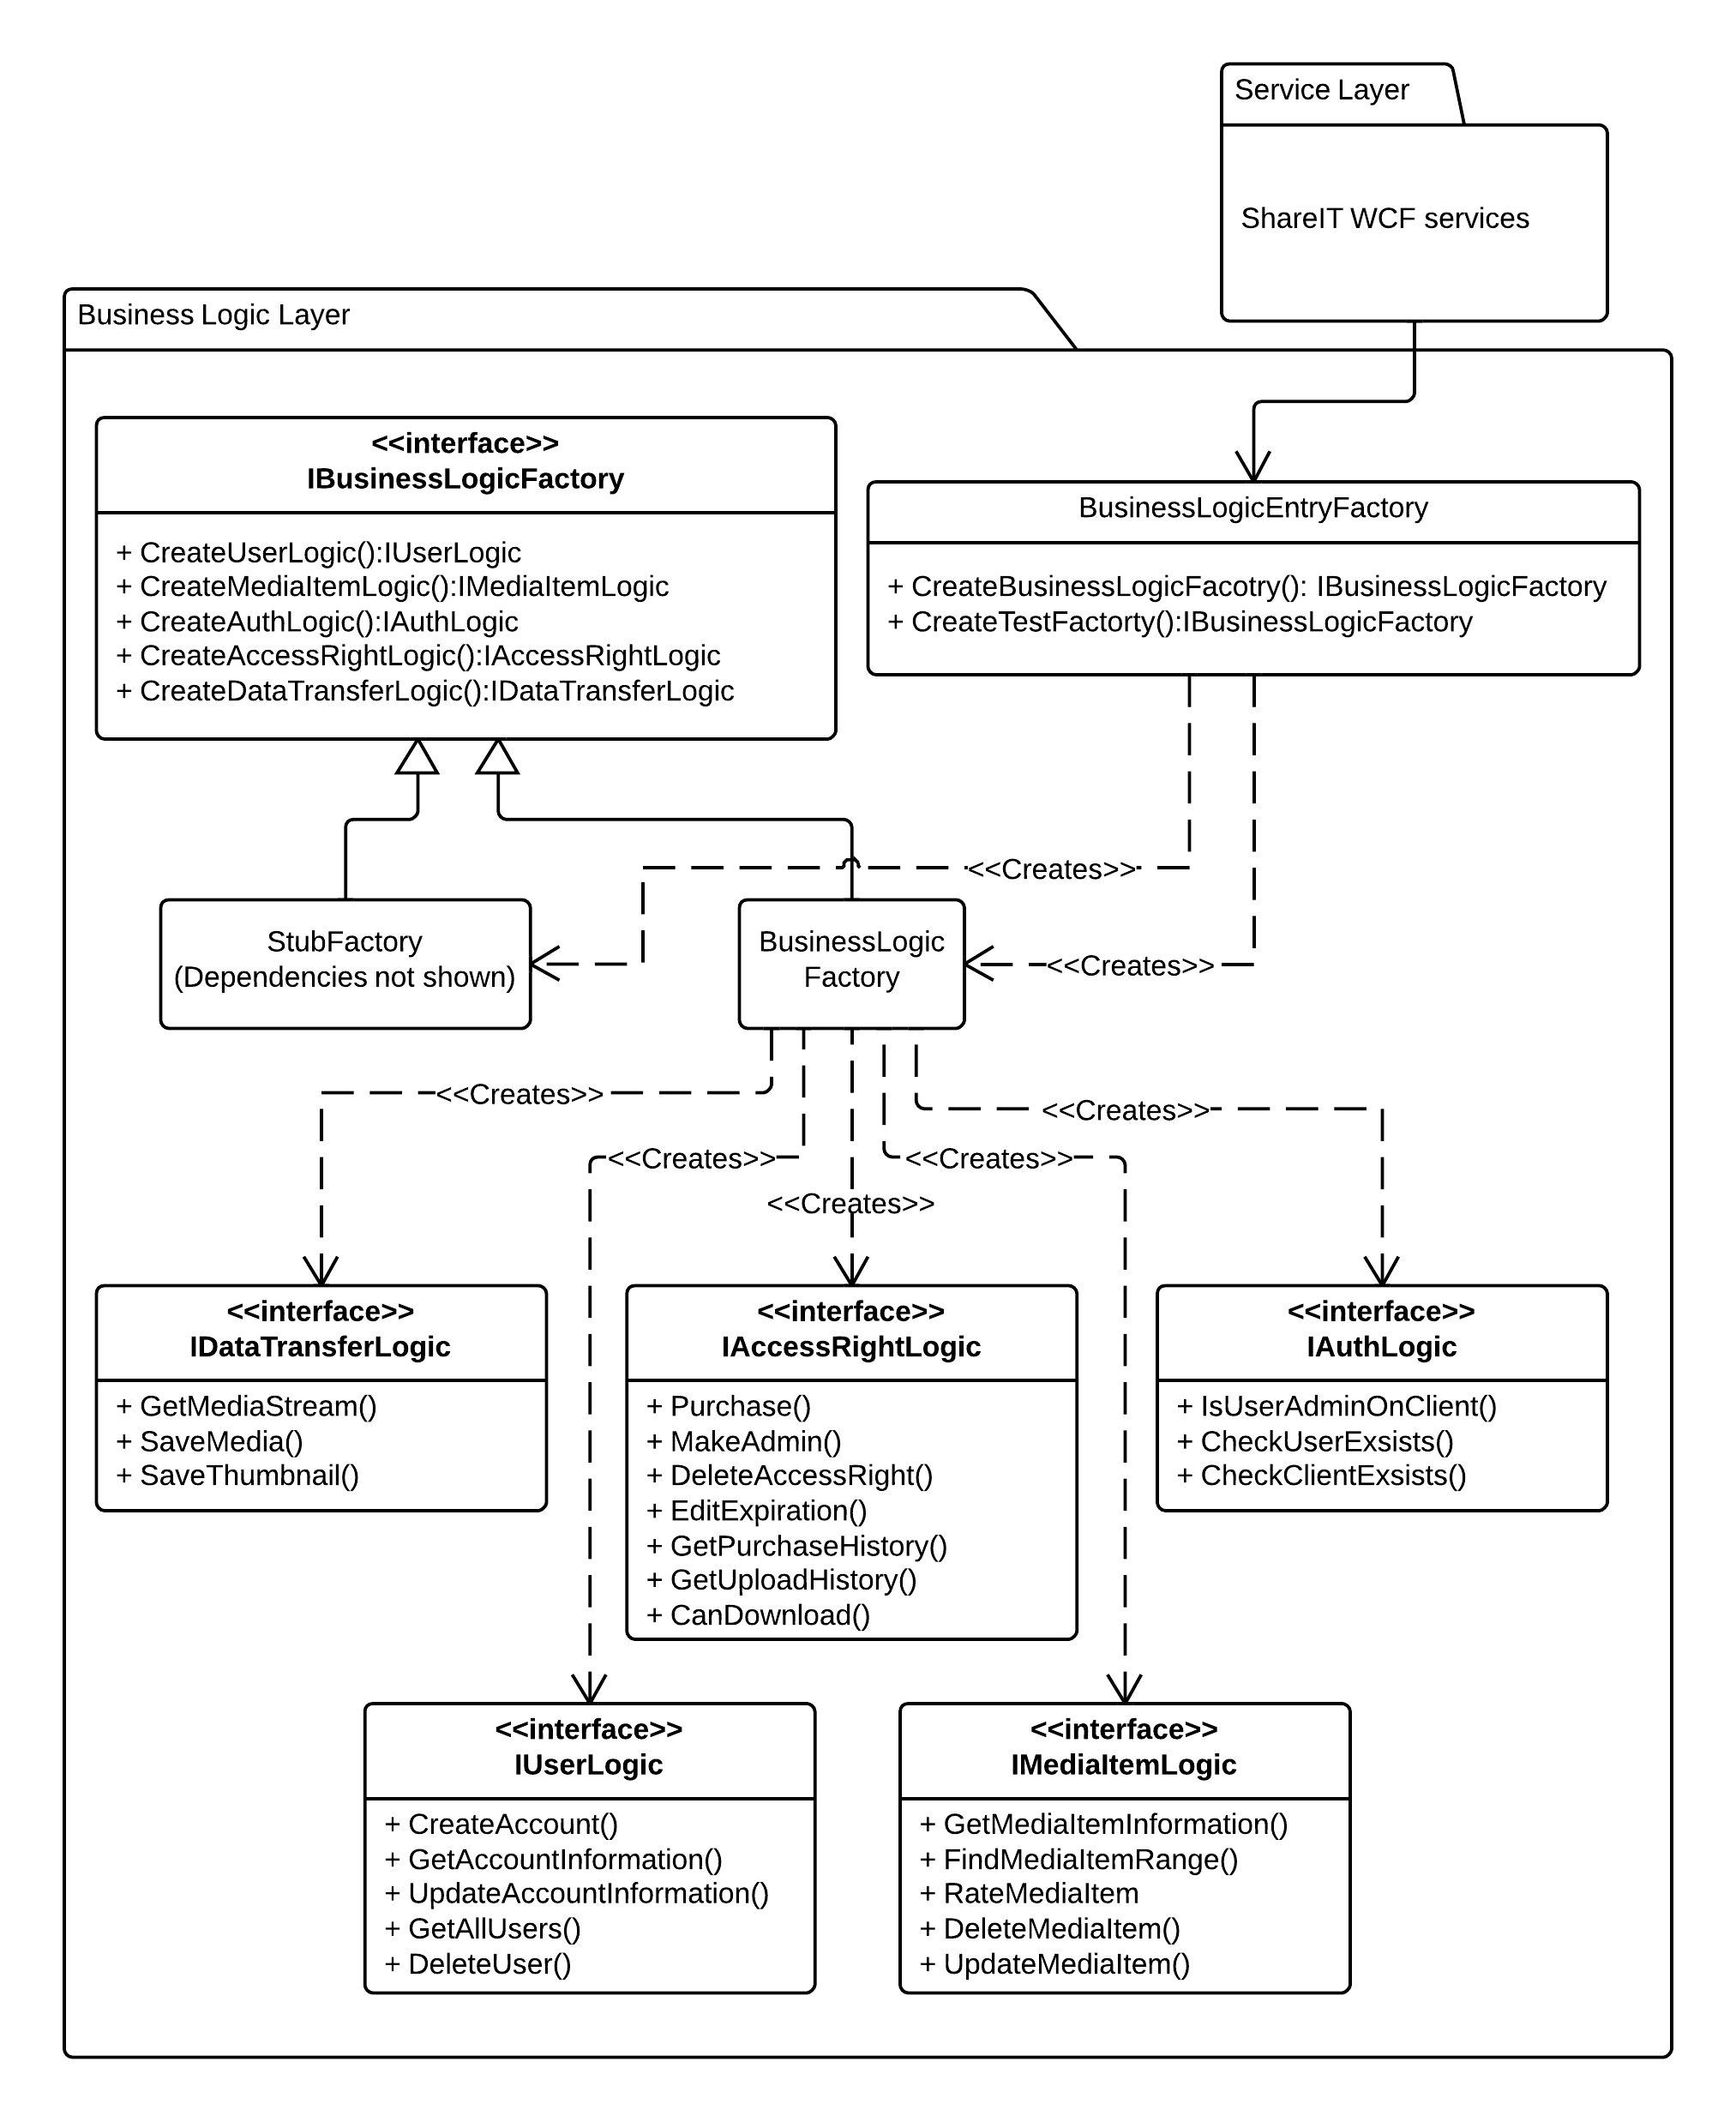
\includegraphics[width=\linewidth]{BLLclassdiagram.png}
\caption{Business Logic Layer class diagram (Not all classes are shown)}
\label{fig:BLLclassdiagram}
\end{figure}




\end{document}